\documentclass[conference]{IEEEtran}
\IEEEoverridecommandlockouts
% The preceding line is only needed to identify funding in the first footnote. If that is unneeded, please comment it out.
\usepackage{cite}
\usepackage{amsmath,amssymb,amsfonts}
\usepackage{algorithmic}
\usepackage{graphicx}
\usepackage{textcomp}
\usepackage{xcolor}
\def\BibTeX{{\rm B\kern-.05em{\sc i\kern-.025em b}\kern-.08em
    T\kern-.1667em\lower.7ex\hbox{E}\kern-.125emX}}
\begin{document}

\title{MFCCs, Chroma Features, and Spectrogram Images for Deepfake Audio Classification Using Machine Learning}

\author{
\IEEEauthorblockN{Nora Bakken, Shavil Singh, Makwana Prashant Lnu, and Tapadhir Das}
\IEEEauthorblockA{Department of Computer Science, University of the Pacific, USA
}
\IEEEauthorblockA{
Email: n\_bakken@u.pacific.edu, tdas@pacific.edu
}}

\maketitle

\begin{abstract}
Deepfake audio detection is critical for combating misinformation in a digital age overrun with dubious media, especially in the new age of AI. This study investigates the performance of different machine learning approaches for classifying deepfake audio, leveraging both Mel-spectrogram representations and Mel-frequency Cepstral Coefficients as audio features. We utilized ResNet50 and VGG16 architectures to classify Mel spectrogram images and applied gradient boosting and support vector machines (SVM) on MFCCs. To SVM, we additionally supplied chroma features, which yielded excellent results.  While ResNet50 and VGG16 achieved high accuracy for original audio spectrograms, their performance degraded significantly on 2-second clips and rerecorded samples. In contrast, gradient boosting on MFCCs achieved over 95\% accuracy, and SVM with chroma features yielded 99\% accuracy across original, normalized, 2-second, and rerecorded datasets. These insights contribute to the development of reliable detection systems for real-world scenarios.
\end{abstract}

\begin{IEEEkeywords}
Mel-frequency cepstral coefficients (MFCCs),
Audio representation,
Convolutional Neural Networks,
Machine Learning,
Adversarial attack protection, 
Cybersecurity,
Spectrogram, 
Chroma Features
\end{IEEEkeywords}


\section{Introduction}

\section{Motivation}

With the rise of artificial intelligence (AI), deepfakes are more prevalent than ever, bringing with them a slough of potential dangers in a variety of areas. Likely the most well-known effect of deepfakes in everyday life is the rise of false media, especially targeting individuals. 

The American Bar Association highlighted a targeted defamation attack involving an audio recording with the voice of a high school principal making racist and antisemitic comments. After the recording spread throughout the school, the principal was in danger of losing his livelihood. He denied making these comments. After a thorough investigation, the local police deemed the recording to have been manipulated using AI \cite{b5}. 

The less talked about consequence of accessible and easy to create deepfakes is the rise of non-consensual explicit deepfake attacks on individuals. These attacks, along with being traumatic to the individual, are expanding the ever-present gender gap at the global level, inflicting consequences at the societal level \cite{b3}.

In the recent United States election, nearly half of American voters stated that deepfakes had an influence on their ballots \cite{b1}. Looking at this problem from a purely monetary perspective, CFO states that 92 percent of companies have experienced financial loss due to a deepfake \cite{b4}. This is a significant economic impact. 

These are just a few of many examples of individuals who have been hurt by deepfake attacks. There is no question about the negative impact that deepfakes actively have on our lives. It is now imperative that an application is developed to reliably identify deepfakes so that fewer individuals are harmed. 

\section{Literature Review}

\section{System Model / Background}

Numerous technologies and algorithms were explored to gather insights on the most effective methods for deepfake audio detection. In this section we will explore the complex features we utilized in our data preprocessing pipeline and discuss the sophisticated machine learning models we employed in our experiments. 

\subsection{MFCCs}

Mel-Frequency Cepstral Coefficients, or MFCCs, are a widely used feature set for speech recognition and other audio processing applications. They are a competitive feature set because they mimic what the human ear perceives \cite{9996362}. The process of extracting MFCCs involves several steps that convert raw audio into a compact representation of its spectral characteristics. One of the key stages in this process is the de-correlation of the log energies from a filter bank. The following quote provides a more detailed explanation of how MFCC coefficients are derived:

\begin{quote}
  "MFCC coefficients are obtained by de-correlating the output log
  energies of a filter bank which consists of triangular filters, linearly spaced on the Mel frequency scale.
  Conventionally an implementation of discrete cosine transform (DCT) known as distributed DCT (DCT - II) is
  used to de-correlate the speech as it is the best available approximation of the Karhunen-Loeve Transform
  (KLT)" \cite{5709752}.
\end{quote}

The resulting vector represents spectral acoustic features as floating-point numbers. These values capture essential characteristics of the audio that aid the model in distinguishing between real and fake samples. The vector's size is flexible and depends on user configuration. 

Generating a vector of MFCC features was an essential step in our preprocessing efforts. A sample rate of 44100 Hz corresponding to a maximum sound frequency of 22050 Hz is usually used for recording sound, because a human can hear sounds ranging from 20 Hz to 20000 Hz \cite{9252126}. In our experiments, we used a sampling rate of 22050 Hz. This is half of the common sample rate for recording sound, and is a common value for sampling rate when generating MFCCs. This resulted in 20 features for each audio sample. These features were then saved to a CSV file, making them available for later model training. These features played a pivotal role in the model's ability to make accurate decisions.

\subsection{Mel-Spectrogram Images}
A Mel-Spectrogram image is an alternative method for visually representing sound. Generally, we see sound visualized as a two-dimensional waveform showing amplitude over time. Figure~\ref{fig:real_waveform} shows an example of a "real" audio sample as a commonly seen waveform. Conversely, figure~\ref{fig:fake_waveform} shows an example of a "fake" audio sample as a waveform. While these representations are helpful, they do not provide enough information for a model to be able to make a decision. 

\begin{figure}
  \centering
  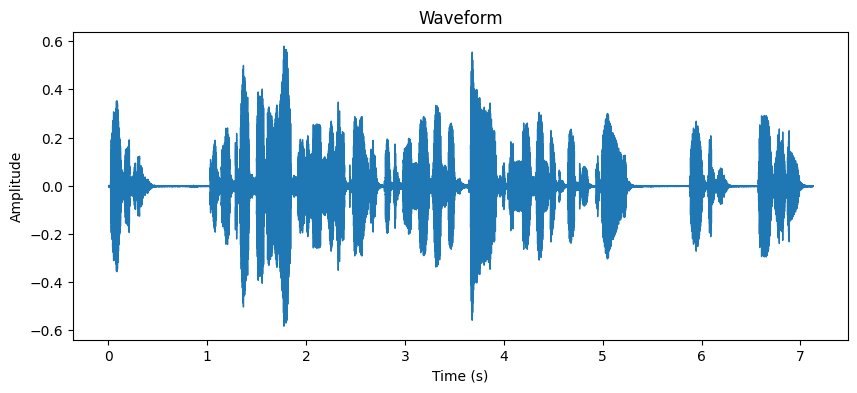
\includegraphics[width=\linewidth]{images/real_waveform.png}
  \caption{Waveform representation of a Real Audio Sample.}
  \label{fig:real_waveform}
\end{figure}

\begin{figure}
  \centering
  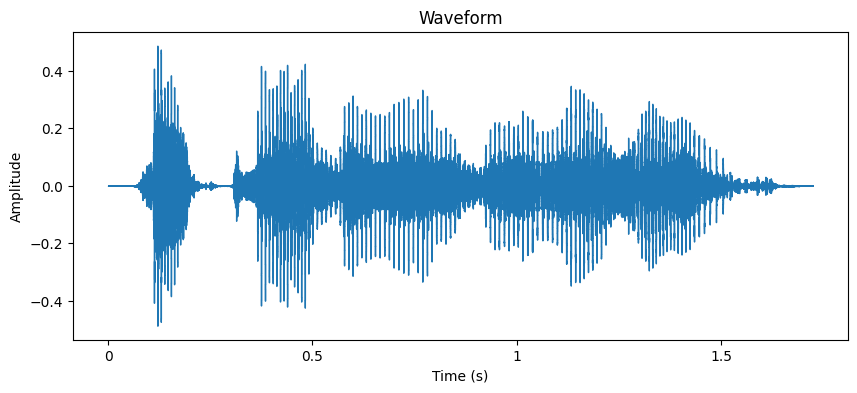
\includegraphics[width=\linewidth]{images/fake_waveform.png}
  \caption{Waveform representation of a Fake Audio Sample.}
  \label{fig:fake_waveform}
\end{figure}

A spectrogram is a representation of an audio signal as its frequency spectrum varies over time. Similar to MFCCs, Mel-Spectrograms are generated by performing a number of transformations on an audio sample, then representing the results as a graph. First, the audio is divided into short segments of time. We used approximately 93 ms segments. Then, a Hamming window is applied to each segment.

The Hamming window can be found with the following formula \cite{9252126}:
\begin{equation}
w(n) = \alpha_0 - (1 - \alpha_0) \cos\left(\frac{2\pi n}{N-1}\right), \quad 0 \leq n \leq N-1
\end{equation}
where \(\alpha_0 = \frac{25}{46}\), and \(N\) is the window length.

Following this operation, Fast Fourier transform (FFT) is applied to calculate the power spectrum of each frame. Lastly, we can obtain the Mel-Spectrogram by applying the Mel filter bank. Frequencies are convered to the Mel scale using the following formula \cite{9252126}:
\begin{equation}
\text{mel} = 2595 \, \lg\left(1 + \frac{f}{700}\right)
\end{equation}

Figure~\ref{fig:real_spectrogram} portrays an example of a "real" audio sample represented as a Mel-spectrogram image. Examining the image, it is clear that it is more information-rich than its two-dimensional counterpart in Figure~\ref{fig:real_waveform}. The additional data represented here is essential to machine learning models as it becomes easier to decide on a classification. Figure~\ref{fig:fake_spectrogram} portrays an example of a "fake" audio sample represented as a Mel-spectrogram image. When comparing this image to figure~\ref{fig:real_spectrogram}, we can see there are some key differences at a glance. These two samples are good examples of their respecive classes. Not all of the generated Mel-spectrogram images in our dataset were so clear cut. Nevertheless, both classes of images encompassed key features on which the model was able to decide. 

\begin{figure}
  \centering
  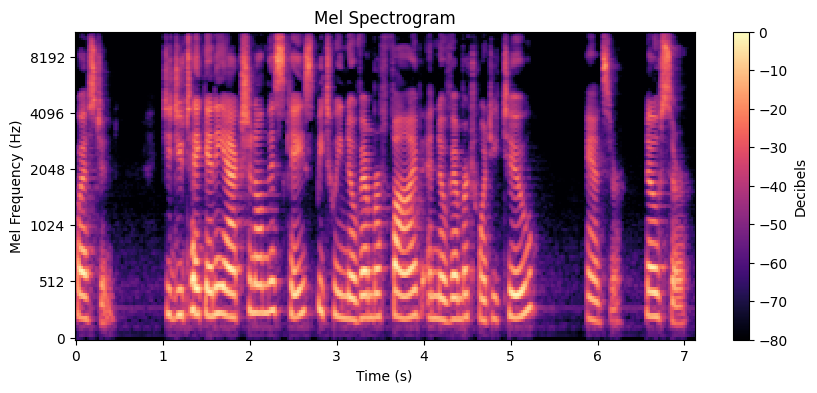
\includegraphics[width=\linewidth]{images/real_spectrogram.png}
  \caption{Spectrogram representation of a Real Audio Sample.}
  \label{fig:real_spectrogram}
\end{figure}

\begin{figure}
  \centering
  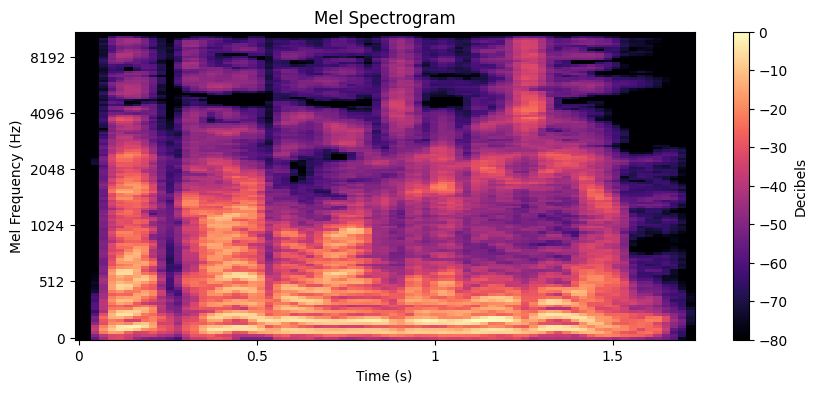
\includegraphics[width=\linewidth]{images/fake_spectrogram.png}
  \caption{Spectrogram representation of a Fake Audio Sample.}
  \label{fig:fake_spectrogram}
\end{figure}

\subsection{Convolutional Neural Networks}
A Convolutional Neural Network, or CNN, is a type of deep learning model specifically designed to process data with a grid-like topology, such as images. It accepts an image with H rows and W columns, and three channels (R, G, B color channels) as input. The input then goes through several layers. First, the Rectified Linear Unit, or ReLU, is a transformation layer. It performs a truncation for each individual element in the input. Next, the input is fed to the convolution layer. This layer searches for edges in the image, and outputs a matrix with these features highlighted. Finally, the pooling layer will reduce the matrix while retaining important features. Then, the process repeats until a classification can be made about the inputted image \cite{wu2017introduction}.

\subsection{Chroma Features}

\section{Methodology}

\subsection{Probably a section about the data here would be good}

\section{Results}

Prof said we need to mention a bit about what algorithms we used here as well as discussing results

\subsection{for-original dataset}

\subsection{for-norm dataset}

\subsection{for-2sec dataset}

\subsection{for-rerec dataset}

\section{Future Work}
Several methods were explored to identify deepfake audio using machine learning; however, despite our promising results, more investigation is needed to compare the impact of chroma features on multiple algorithms besides SVM. We would also like to work on improving the accuracy of all approaches on the \textit{for-2sec} and \textit{for-rerec} datasets. Lastly, it could be meaningful to explore other audio representations other than MFCCs and Mel-Spectrograms to consider features which these representations may not encompass. 

\section{Conclusion}

\section*{Acknowledgment}

\bibliographystyle{IEEEtran}
\bibliography{sample} % Reference to .bib file

\end{document}
